% Created by tikzDevice version 0.8.1 on 2015-06-10 21:23:04
% !TEX encoding = UTF-8 Unicode
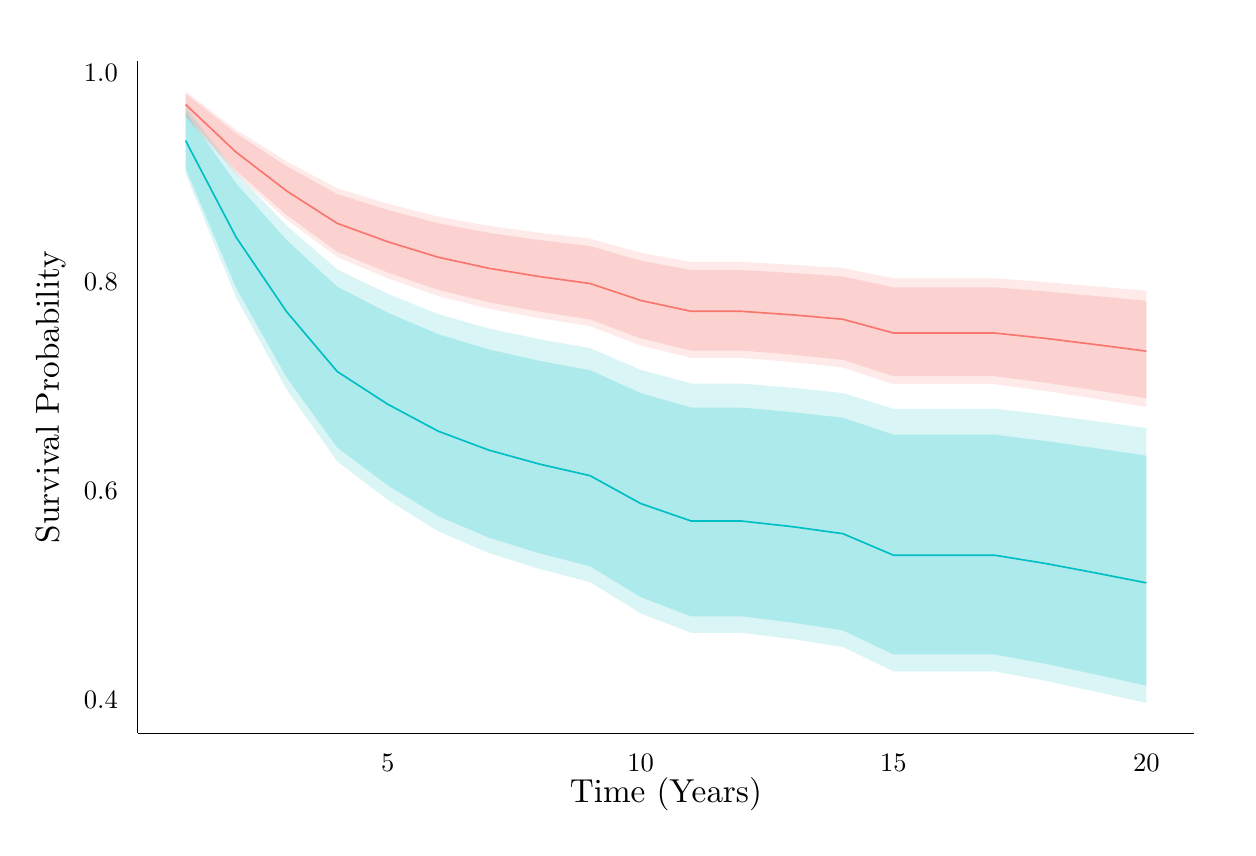
\begin{tikzpicture}[x=1pt,y=1pt]
\definecolor{fillColor}{RGB}{255,255,255}
\path[use as bounding box,fill=fillColor,fill opacity=0.00] (0,0) rectangle (433.62,289.08);
\begin{scope}
\path[clip] (  0.00,  0.00) rectangle (433.62,289.08);
\definecolor{drawColor}{RGB}{255,255,255}
\definecolor{fillColor}{RGB}{255,255,255}

\path[draw=drawColor,line width= 0.6pt,line join=round,line cap=round,fill=fillColor] (  0.00,  0.00) rectangle (433.62,289.08);
\end{scope}
\begin{scope}
\path[clip] ( 39.69, 34.03) rectangle (421.57,277.03);
\definecolor{fillColor}{RGB}{255,255,255}

\path[fill=fillColor] ( 39.69, 34.03) rectangle (421.58,277.03);
\definecolor{drawColor}{RGB}{248,118,109}

\path[draw=drawColor,line width= 0.6pt,line join=round] ( 57.05,261.32) --
	( 75.32,244.08) --
	( 93.59,230.08) --
	(111.86,218.35) --
	(130.13,211.71) --
	(148.41,206.11) --
	(166.68,202.12) --
	(184.95,199.13) --
	(203.22,196.63) --
	(221.49,190.52) --
	(239.77,186.58) --
	(258.04,186.58) --
	(276.31,185.31) --
	(294.58,183.71) --
	(312.86,178.74) --
	(331.13,178.74) --
	(349.40,178.74) --
	(367.67,176.82) --
	(385.94,174.56) --
	(404.22,172.20);
\definecolor{drawColor}{RGB}{0,191,196}

\path[draw=drawColor,line width= 0.6pt,line join=round] ( 57.05,248.29) --
	( 75.32,213.35) --
	( 93.59,186.41) --
	(111.86,164.83) --
	(130.13,152.99) --
	(148.41,143.24) --
	(166.68,136.42) --
	(184.95,131.37) --
	(203.22,127.19) --
	(221.49,117.14) --
	(239.77,110.80) --
	(258.04,110.80) --
	(276.31,108.77) --
	(294.58,106.23) --
	(312.86, 98.45) --
	(331.13, 98.45) --
	(349.40, 98.45) --
	(367.67, 95.49) --
	(385.94, 92.05) --
	(404.22, 88.46);
\definecolor{fillColor}{RGB}{248,118,109}

\path[fill=fillColor,fill opacity=0.15] ( 57.05,265.99) --
	( 75.32,252.20) --
	( 93.59,240.74) --
	(111.86,231.01) --
	(130.13,225.45) --
	(148.41,220.77) --
	(166.68,217.45) --
	(184.95,214.94) --
	(203.22,212.84) --
	(221.49,207.73) --
	(239.77,204.43) --
	(258.04,204.43) --
	(276.31,203.42) --
	(294.58,202.21) --
	(312.86,198.53) --
	(331.13,198.53) --
	(349.40,198.53) --
	(367.67,197.17) --
	(385.94,195.60) --
	(404.22,193.96) --
	(404.22,152.02) --
	(385.94,155.00) --
	(367.67,157.83) --
	(349.40,160.23) --
	(331.13,160.23) --
	(312.86,160.23) --
	(294.58,166.32) --
	(276.31,168.26) --
	(258.04,169.76) --
	(239.77,169.76) --
	(221.49,174.25) --
	(203.22,181.25) --
	(184.95,184.11) --
	(166.68,187.53) --
	(148.41,192.10) --
	(130.13,198.53) --
	(111.86,206.18) --
	( 93.59,219.74) --
	( 75.32,236.14) --
	( 57.05,256.70) --
	cycle;
\definecolor{fillColor}{RGB}{0,191,196}

\path[fill=fillColor,fill opacity=0.15] ( 57.05,260.52) --
	( 75.32,236.66) --
	( 93.59,217.51) --
	(111.86,201.70) --
	(130.13,192.89) --
	(148.41,185.54) --
	(166.68,180.36) --
	(184.95,176.49) --
	(203.22,173.28) --
	(221.49,165.46) --
	(239.77,160.49) --
	(258.04,160.49) --
	(276.31,158.93) --
	(294.58,157.04) --
	(312.86,151.36) --
	(331.13,151.36) --
	(349.40,151.36) --
	(367.67,149.27) --
	(385.94,146.88) --
	(404.22,144.40) --
	(404.22, 45.08) --
	(385.94, 49.16) --
	(367.67, 53.09) --
	(349.40, 56.47) --
	(331.13, 56.47) --
	(312.86, 56.47) --
	(294.58, 65.28) --
	(276.31, 68.15) --
	(258.04, 70.40) --
	(239.77, 70.40) --
	(221.49, 77.46) --
	(203.22, 88.74) --
	(184.95, 93.48) --
	(166.68, 99.25) --
	(148.41,107.10) --
	(130.13,118.44) --
	(111.86,132.39) --
	( 93.59,158.31) --
	( 75.32,191.63) --
	( 57.05,236.46) --
	cycle;
\definecolor{fillColor}{RGB}{248,118,109}

\path[fill=fillColor,fill opacity=0.20] ( 57.05,265.23) --
	( 75.32,250.88) --
	( 93.59,239.01) --
	(111.86,228.94) --
	(130.13,223.20) --
	(148.41,218.37) --
	(166.68,214.93) --
	(184.95,212.34) --
	(203.22,210.18) --
	(221.49,204.89) --
	(239.77,201.49) --
	(258.04,201.49) --
	(276.31,200.43) --
	(294.58,199.16) --
	(312.86,195.26) --
	(331.13,195.26) --
	(349.40,195.26) --
	(367.67,193.80) --
	(385.94,192.11) --
	(404.22,190.35) --
	(404.22,155.16) --
	(385.94,158.05) --
	(367.67,160.79) --
	(349.40,163.12) --
	(331.13,163.12) --
	(312.86,163.12) --
	(294.58,169.04) --
	(276.31,170.93) --
	(258.04,172.39) --
	(239.77,172.39) --
	(221.49,176.81) --
	(203.22,183.67) --
	(184.95,186.47) --
	(166.68,189.83) --
	(148.41,194.31) --
	(130.13,200.61) --
	(111.86,208.10) --
	( 93.59,221.38) --
	( 75.32,237.40) --
	( 57.05,257.44) --
	cycle;
\definecolor{fillColor}{RGB}{0,191,196}

\path[fill=fillColor,fill opacity=0.20] ( 57.05,258.52) --
	( 75.32,232.80) --
	( 93.59,212.30) --
	(111.86,195.45) --
	(130.13,186.08) --
	(148.41,178.28) --
	(166.68,172.79) --
	(184.95,168.69) --
	(203.22,165.30) --
	(221.49,157.03) --
	(239.77,151.79) --
	(258.04,151.79) --
	(276.31,150.14) --
	(294.58,148.11) --
	(312.86,142.01) --
	(331.13,142.01) --
	(349.40,142.01) --
	(367.67,139.74) --
	(385.94,137.13) --
	(404.22,134.42) --
	(404.22, 51.33) --
	(385.94, 55.36) --
	(367.67, 59.25) --
	(349.40, 62.58) --
	(331.13, 62.58) --
	(312.86, 62.58) --
	(294.58, 71.28) --
	(276.31, 74.11) --
	(258.04, 76.35) --
	(239.77, 76.35) --
	(221.49, 83.33) --
	(203.22, 94.46) --
	(184.95, 99.14) --
	(166.68,104.81) --
	(148.41,112.53) --
	(130.13,123.67) --
	(111.86,137.33) --
	( 93.59,162.63) --
	( 75.32,195.02) --
	( 57.05,238.34) --
	cycle;
\end{scope}
\begin{scope}
\path[clip] (  0.00,  0.00) rectangle (433.62,289.08);
\definecolor{drawColor}{RGB}{0,0,0}

\path[draw=drawColor,line width= 0.6pt,line join=round] ( 39.69, 34.03) --
	( 39.69,277.03);
\end{scope}
\begin{scope}
\path[clip] (  0.00,  0.00) rectangle (433.62,289.08);
\definecolor{drawColor}{RGB}{0,0,0}

\node[text=drawColor,anchor=base east,inner sep=0pt, outer sep=0pt, scale=  0.96] at ( 32.57, 42.91) {0.4};

\node[text=drawColor,anchor=base east,inner sep=0pt, outer sep=0pt, scale=  0.96] at ( 32.57,118.48) {0.6};

\node[text=drawColor,anchor=base east,inner sep=0pt, outer sep=0pt, scale=  0.96] at ( 32.57,194.05) {0.8};

\node[text=drawColor,anchor=base east,inner sep=0pt, outer sep=0pt, scale=  0.96] at ( 32.57,269.62) {1.0};
\end{scope}
\begin{scope}
\path[clip] (  0.00,  0.00) rectangle (433.62,289.08);
\definecolor{drawColor}{RGB}{0,0,0}

\path[draw=drawColor,line width= 0.6pt,line join=round] ( 39.69, 34.03) --
	(421.57, 34.03);
\end{scope}
\begin{scope}
\path[clip] (  0.00,  0.00) rectangle (433.62,289.08);
\definecolor{drawColor}{RGB}{0,0,0}

\node[text=drawColor,anchor=base,inner sep=0pt, outer sep=0pt, scale=  0.96] at (130.13, 20.31) {5};

\node[text=drawColor,anchor=base,inner sep=0pt, outer sep=0pt, scale=  0.96] at (221.49, 20.31) {10};

\node[text=drawColor,anchor=base,inner sep=0pt, outer sep=0pt, scale=  0.96] at (312.86, 20.31) {15};

\node[text=drawColor,anchor=base,inner sep=0pt, outer sep=0pt, scale=  0.96] at (404.22, 20.31) {20};
\end{scope}
\begin{scope}
\path[clip] (  0.00,  0.00) rectangle (433.62,289.08);
\definecolor{drawColor}{RGB}{0,0,0}

\node[text=drawColor,anchor=base,inner sep=0pt, outer sep=0pt, scale=  1.20] at (230.63,  9.03) {Time (Years)};
\end{scope}
\begin{scope}
\path[clip] (  0.00,  0.00) rectangle (433.62,289.08);
\definecolor{drawColor}{RGB}{0,0,0}

\node[text=drawColor,rotate= 90.00,anchor=base,inner sep=0pt, outer sep=0pt, scale=  1.20] at ( 11.28,155.53) {Survival Probability};
\end{scope}
\end{tikzpicture}
